\subsection{Übersicht}\label{übersicht}
Die Komponente “App und Datenbankhandling” besteht zum wesentlich aus diesen drei Unterkomponenten.  

\begin{figure}[h]
 \centering
 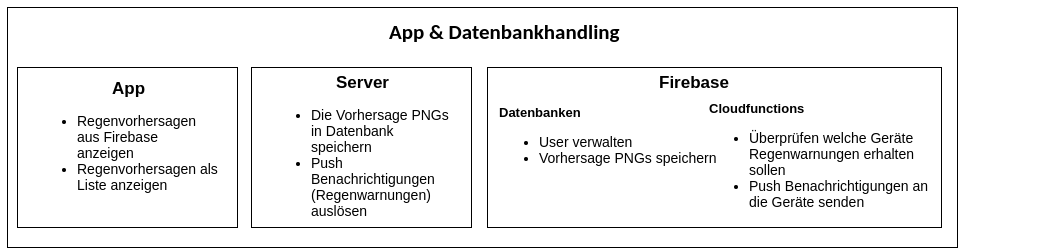
\includegraphics[width=1\textwidth,angle=0]{abb/app_datenbank_komponente_uebersicht}
 \caption[Komponentenübersicht App und Datenbankhandling]{Die Komponente App und Datenbankhandling}
\label{fig:Beschreibung}
\end{figure}

Die App dient zur Visualisierung der Daten und macht somit die Regenvorhersagen für den Endnutzer brauchbar. 
Auf dem Server werden die Vorhersagen berechnet und in dem für dieses Kapitel relevanten Teil
für die App zur Verfügung gestellt. 
Die Firebase verbindet den Server mit der App und erfüllt dabei im wesentlichen zwei verschiedene Aufgaben. 
Sie stellt die Regenvorhersagen als PNG für die App zur Verfügung und übernimmt das  Senden der Pushbenachrichtigungen,
welche für die Regenwarnungen gebraucht werden.
 
